
\usetikzlibrary{shapes, arrows.meta, positioning, fit, decorations.pathreplacing,
decorations.pathmorphing, decorations.shapes, calc}

\tikzset{dada2/.style={draw, fill=green!10, align=center}}
\tikzset{vsearch/.style={draw, fill=red!20, align=center}}
\tikzset{usearch/.style={draw, fill=magenta!10, align=center}}
\tikzset{cutadapt/.style={draw, fill=cyan!10, align=center}}
\tikzset{protax/.style={draw, fill=blue!15, align=center}}
\tikzset{protax_or_vsearch/.style={draw, shade, right color=blue!15, left color=red!20, align=center}}
\tikzset{protax_or_usearch/.style={draw, shade, right color=blue!15, left color=magenta!10, align=center}}
\tikzset{infernal/.style={draw, fill=orange!15, align=center}}
\tikzset{new/.style={draw, fill=yellow!10, align=center}}
\tikzset{data/.style={align=center}}
\tikzset{key/.style={minimum width=35mm}}

% \tikzset{parallel/.style={dotted, line width=1pt}}
\tikzset{parallel/.style={fill=gray!20, rounded corners}}
\tikzset{paired reads/.style={line width = 1pt, double distance=0.5pt,decorate, decoration={snake, amplitude=0.75pt, segment length = 3pt, post=lineto, post length=2mm}}}
\tikzset{single reads/.style={decorate, decoration={snake, amplitude=0.75pt, segment length = 3pt, post=lineto, post length=2mm}}}
\tikzset{table/.style={line width=1pt}}
\tikzset{taxonomy/.style={double distance=0.5pt}}

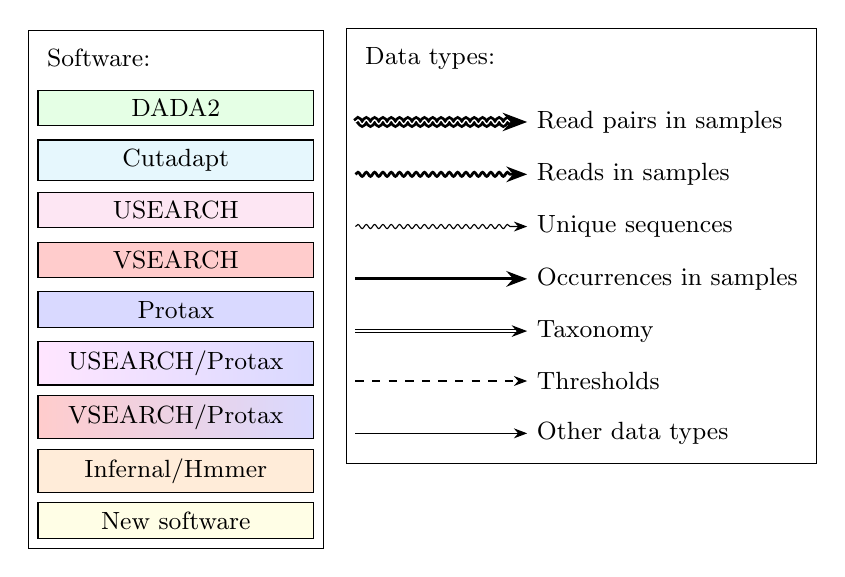
\begin{tikzpicture}[font=\small,node distance=4mm]
\node (softwarekey) {Software:};
\node[below= of softwarekey.west,anchor = north west, dada2, key] (dada2key) {DADA2};
\node[below= of dada2key.west, anchor=north west, cutadapt, key] (cutadaptkey) {Cutadapt};
\node[below= of cutadaptkey.west, anchor=north west, usearch, key] (usearchkey) {USEARCH};
\node[below= of usearchkey.west, anchor=north west, vsearch, key] (vsearchkey) {VSEARCH};
\node[below= of vsearchkey.west, anchor=north west, protax, key] (protaxkey) {Protax};
\node[below= of protaxkey.west, anchor=north west, protax_or_usearch, key] (protaxusearchkey) {USEARCH/Protax};
\node[below= of protaxusearchkey.west, anchor=north west, protax_or_vsearch, key] (protaxvsearchkey) {VSEARCH/Protax};
\node[below= of protaxvsearchkey.west, anchor=north west, infernal, key] (infernalkey) {Infernal/Hmmer};
\node[below= of infernalkey.west, anchor=north west, new, key] (newkey) {New software};
\node[draw, fit=(softwarekey) (dada2key) (newkey) (infernalkey) (protaxusearchkey) (protaxvsearchkey)](softwareframe){};

\node[right = of $(softwareframe.east |- softwarekey)$] (datakey) {Data types:};
\node[below right = of datakey] (pairedkey) {Read pairs in samples};
\node[below = of pairedkey.west, anchor=north west] (readkey) {Reads in samples};
\node[below = of readkey.west, anchor=north west] (sequencekey) {Unique sequences};
\node[below = of sequencekey.west, anchor=north west] (tablekey) {Occurrences in samples};
\node[below = of tablekey.west, anchor=north west] (taxonomykey) {Taxonomy};
\node[below = of taxonomykey.west, anchor=north west] (thresholdkey) {Thresholds};
\node[below = of thresholdkey.west, anchor = north west] (otherkey) {Other data types};
\node[draw, fit=(datakey) (pairedkey) (readkey) (sequencekey) (tablekey) (thresholdkey) (otherkey)] (dataframe){};

\draw[-Stealth, paired reads] (datakey.west |- pairedkey) -- (pairedkey);
\draw[-Stealth, single reads, table] (datakey.west |- readkey) -- (readkey);
\draw[-Stealth, single reads] (datakey.west |- sequencekey) -- (sequencekey);
\draw[-Stealth, table] (datakey.west |- tablekey) -- (tablekey);
\draw[-Stealth, taxonomy] (datakey.west |- taxonomykey) -- (taxonomykey);
\draw[-Stealth, dashed] (datakey.west |- thresholdkey) -- (thresholdkey);
\draw[-Stealth] (datakey.west |- otherkey) -- (otherkey);
\end{tikzpicture}
